\documentclass[a4paper, 11pt]{article}
\usepackage{comment} % enables the use of multi-line comments (\ifx \fi) 
\usepackage{fullpage} % changes the margin
\usepackage{graphicx}
\usepackage{subfigure}
\usepackage{amsmath}
\usepackage{amsfonts}



\begin{document}
\noindent
\large\textbf{Homework 3} \hfill \textbf{Yen-Lin Chen} \\
\normalsize ECE 5412 \hfill yc2253@cornell.edu \\
Fall 2019 \hfill Due: 11/30/19\\

\section*{Problem 49}

Let $f = \mathbf{E}[(X-g(Y))'R(X-g(Y))]$ and we would like to find $g(Y)$ that minimizes $f$. 

\begin{equation}
\begin{split}
f = & \mathbf{E}[X'RX - g(Y)'RX - X'Rg(Y) + g(Y)'Rg(Y)]\\
\frac{\partial f}{\partial g(Y)} & = 0 = \mathbf{E}[-2RX + 2Rg(Y)]\\
\Longrightarrow & \mathbf{E}[RX] = \mathbf{E}[Rg(Y)]
\end{split}
\end{equation}

Using the iterated expectations: $\mathbf{E}[g(X,Y)] = \mathbf{E}_Y\{\mathbf{E}_X[g(X,Y)|Y]\}$

\begin{equation}
\mathbf{E}_Y\left\{ \mathbf{E}_X [RX | Y] \right\} = \mathbf{E}_Y\left\{ \mathbf{E}_X [Rg(Y) | Y] \right\} = \mathbf{E}_Y[Rg(Y)]
\end{equation}

\begin{equation}
R\mathbf{E}_Y\{\mathbf{E}_X[X|Y] \} = R\mathbf{E}_Y[g(Y)]
\end{equation}


Since $R$ is positive definite, $R^{-1}$ exists. Therefore, $\mathbf{E}_X[X|Y] = g(Y)$


\section*{Problem 51}

Suppose $\pi_1 = P'\pi_0 = (p_1, p_2)'$. Since $y_1 = x_1 + v_1$ where $v_1 \sim N(0,1 )$, we have $y_1|x_1 \sim N(y_1-x_1, 1)$. 
\begin{equation}
P(y_1|x_1) = \frac{1}{\sqrt{2\pi}}\exp\left[{-\frac{1}{2}(y_1-x_1)^2}\right]
\end{equation}
From the Bayes rule, 

\begin{equation}
P(x_1|y_1) = \frac{P(y_1|x_1)P(x_1)}{\sum_{x_1}P(y_1|x_1)P(x_1)}
\end{equation}
where $P(x_1=1) = p_1$ and $P(x_2=2) = p_2$.

\begin{equation}
\begin{split}
P(x_1 = 1|y_1) & = \frac{p_1\exp\left[{-\frac{1}{2}(y_1-1)^2}\right]}{p_1\exp\left[{-\frac{1}{2}(y_1-1)^2}\right] + p_2\exp\left[{-\frac{1}{2}(y_1-2)^2}\right]} \\
P(x_1 = 2|y_1) & = \frac{p_2\exp\left[{-\frac{1}{2}(y_1-2)^2}\right]}{p_1\exp\left[{-\frac{1}{2}(y_1-1)^2}\right] + p_2\exp\left[{-\frac{1}{2}(y_1-2)^2}\right]}
\end{split}
\end{equation}
We can simplify Eq. (6) further as the following

\begin{equation}
\begin{split}
P(x_1 = 1|y_1) & = \frac{p_1\exp\left[{-\frac{1}{2}(2y-3)}\right]}{p_1\exp\left[{-\frac{1}{2}(2y-3)}\right] + p_2} \\
P(x_1 = 2|y_1) & = \frac{p_2}{p_1\exp\left[{-\frac{1}{2}(2y-3)}\right] + p_2}
\end{split}
\end{equation}


\section*{Problem 54}

The transition probability of the Markov Chain is 

\begin{equation}
P_{ij} = P(X=j|X=i) = \frac{b_j}{b_i + b_j}Q_{ij}
\end{equation}
Since $Q_{ij} = Q_{ji}$ and $b_i > 0$ $\forall i=1,2,\dots, N$, we want to find the stationary distribution $\pi_\infty$ that satisfies $P_{ij}\pi_\infty(i) = P_{ji}\pi_\infty(j)$, i.e.

\begin{equation}
\frac{b_j}{b_i + b_j}Q_{ij}\pi_\infty(i) = \frac{b_i}{b_i + b_j}Q_{ji}\pi_\infty(j)
\end{equation}
Suppose $Q_{ij}=Q_{ji}\neq 0$, we have
\begin{equation}
\frac{\pi_\infty(i)}{b_i} = \frac{\pi_\infty(j)}{b_j}
\end{equation}
Therefore, with stationary distribution $\pi_infty(i) \propto b_i$, this Markov Chain satisfies the balanced equation and is reversible. 


\section*{Problem 55}


Let $X\in\mathbb{R}^n$ be the data to be classified into binary class $Y \in \{0, 1\}$. The naive Bayes classifier is 
\begin{equation}
g(X) = \text{arg}\max_Y P(Y|X)
\end{equation}
Given data $X$, the naive Bayes classifier outputs $1$ if $P(Y=1|X) > P(Y=0|X)$. The linear discriminant analysis (LDA) is a classifier based on constructing a hyper-plane in $\mathbb{R}^n$. 

We first explore the parametric case where $P(X|Y)\sim N(\mu_Y, \Sigma)$ with prior $\pi(Y=0)$ and $\pi(Y=1)$. Then the naive Bayes classifier is comparing the conditional probability of $P(Y=0|X)$ and $P(Y=1|X)$, i.e.
\begin{equation}
\begin{split}
g(X) & = \text{arg}\max_{Y\in\{0,1\}}\left[\log\pi(Y) - \frac{1}{2}(X - \mu_Y)'\Sigma^{-1}(X - \mu_Y) \right]\\
 & = \text{arg}\max_{Y\in\{0,1\}}\left[\log\pi(Y) + \frac{1}{2}(2\mu_Y\Sigma^{-1}X - \mu_Y'\Sigma^{-1}\mu_Y) \right]
\end{split}
\end{equation}

The LDA hyper-plane is $P(Y=0|X) = P(Y=1|X) = \frac{1}{2}$ and substituting $\mu$, $\Sigma$ and $\pi$ with the empirical estimators $\hat{\mu}$, $\hat{\Sigma}$ and $\hat{\pi}$:
\begin{equation}
\log\hat{\pi}(Y=0) + \frac{1}{2}(2\hat{\mu_0}'\hat{\Sigma}^{-1}X - \hat{\mu_0}'\hat{\Sigma}^{-1}\hat{\mu_0}) = \log\hat{\pi}(Y=1) + \frac{1}{2}(2\hat{\mu_1}'\hat{\Sigma}^{-1}X - \hat{\mu_1}'\hat{\Sigma}^{-1}\hat{\mu_1})
\end{equation}

We use the \textit{fisheriris.mat} data set to illustrate the performance of parametric LDA. The data set contains three classes: \textit{setosa}, \textit{versicolor} and \textit{virginica} with $n = 4$ and $50$ observation for each class. We remove the \textit{virginica} data to make it a binary classification problem with $Y = 0$ for \textit{setosa} and $Y=1$ for \textit{versicolor}. Therefore, $\hat{\pi}(Y=0) = \hat{\pi}(Y=1) = \frac{1}{2}$. Eq. (13) is simplified as follows
\begin{equation}
\begin{split}
2\hat{\mu_0}'\hat{\Sigma}^{-1}X - \hat{\mu_0}'\hat{\Sigma}^{-1}\hat{\mu_0} & = 2\hat{\mu_1}'\hat{\Sigma}^{-1}X - \hat{\mu_1}'\hat{\Sigma}^{-1}\hat{\mu_1}\\
\iff 2(\hat{\mu_0} - \hat{\mu_1})'\hat{\Sigma}^{-1}X & = \hat{\mu_0}'\hat{\Sigma}^{-1}\hat{\mu_0} - \hat{\mu_1}'\hat{\Sigma}^{-1}\hat{\mu_1}
\end{split}
\end{equation}

Secondly, we can use a semi-parametric model: 
\begin{equation}
P(Y=1|X=x) = \frac{e^{\alpha+\beta'x}}{e^{\alpha+\beta'x}+1} = \frac{1}{1+e^{-(\alpha+\beta'x)}}
\end{equation}
We can use the maximum likelihood to estimate $\alpha$ and $\beta$ using the data. The likelihood function is
\begin{equation}
L = \prod_{i=1}^nP(x_i)^{y_i}(1-P(x_i))^{(1-y_i)}
\end{equation}
\begin{equation}
l = \log L = \sum_{i=1}^n\log{(1-P(x_i))} + \sum_{i=1}^n y_i\log{\left(\frac{P(x_i)}{1-P(x_i)} \right)}
\end{equation}
where $P(x_i) = P(Y=1|X=x_i)$. Eq. (17) does not have a close form expression so we have to use numerical optimization to estimate $\alpha$ and $\beta$. Fortunately, we have the gradient of the target function $l$:
\begin{equation}
\begin{split}
\frac{\partial l}{\partial \alpha} & = \sum_{i=1}^n (y_i - P(x_i))\\
\frac{\partial l}{\partial \beta_j} & = \sum_{i=1}^n (y_i - P(x_i))x_{ij}\\
\end{split}
\end{equation}

\begin{figure}
	\begin{center}
		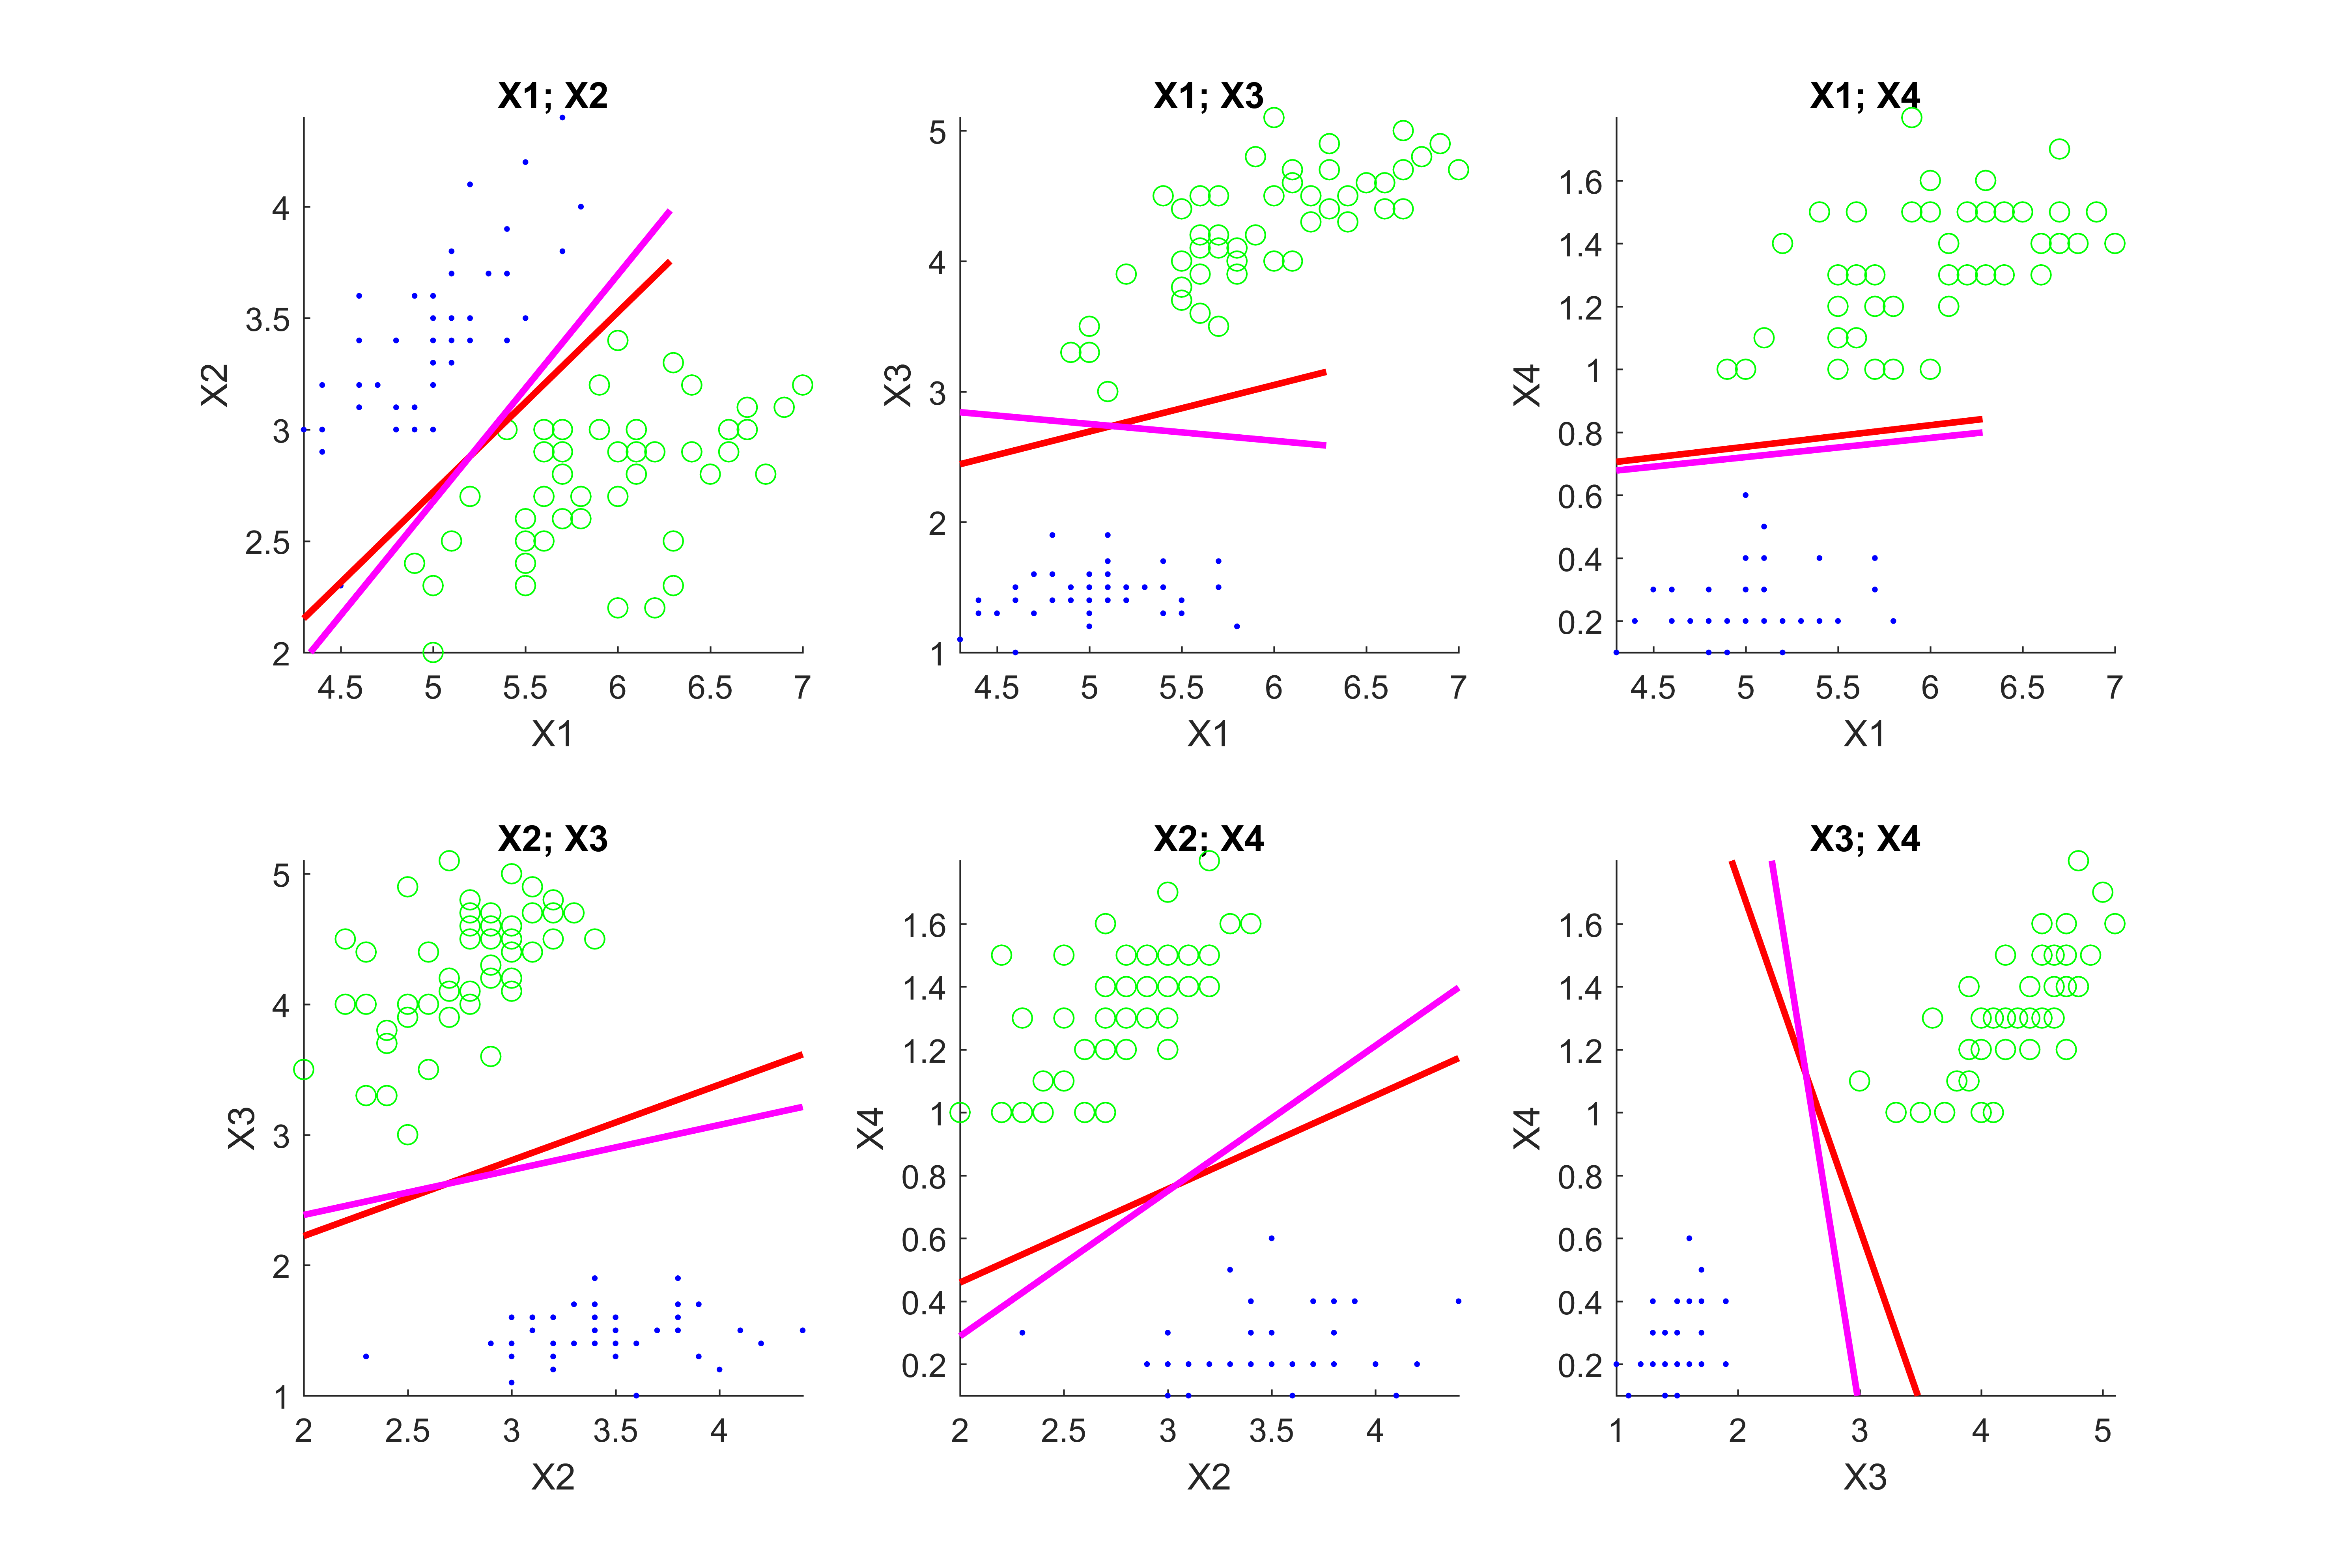
\includegraphics[width=6in]{p55.png}
		\caption{Problem 55: The naive Bayes and logistic classifiers are shown as red and magenta lines.}
	\end{center}
\end{figure}


The binary classification results are shown in Fig. 1 with the naive Bayes and logistic classifiers being the red and magenta lines respectively. 




\section*{Problem 57}

Please see the final section for the short report. 


\section*{Problem 58}





\section*{Problem 59}





\section*{Problem 61}




\section*{Problem 62}




\section*{Attachments}
\textit{p37.m, ar2simulate.m, arestimate.m, rls.m}



\end{document}
